\documentclass[12pt,italian]{article}
\usepackage[T1]{fontenc}
\usepackage{babel}
\usepackage[utf8]{inputenc}
\usepackage{enumitem}
\usepackage{subfiles}
\usepackage{multirow}
\usepackage{color}
\usepackage{titlesec}
\usepackage{longtable}
\usepackage{xcolor,colortbl}
\usepackage[hidelinks]{hyperref}
\usepackage{graphicx}
\usepackage{amsmath}
\usepackage{mdframed}
\usepackage{listings}
\usepackage{minted}

\usepackage[a4paper,width=180mm,top=25mm,bottom=25mm]{geometry}
\usepackage{afterpage}
\usepackage{array,ragged2e}
\usepackage{booktabs}

\graphicspath{{./immagini/}}

\definecolor{LightGray}{gray}{0.9}

\definecolor{codegreen}{rgb}{0,0.6,0}
\definecolor{codegray}{rgb}{0.5,0.5,0.5}
\definecolor{codepurple}{rgb}{0.58,0,0.82}
\definecolor{backcolour}{rgb}{0.95,0.95,0.92}

\newcolumntype{P}[1]{>{\RaggedRight\arraybackslash}p{#1}}
\newlist{tabitem}{itemize}{1}
\setlist[tabitem]{nosep,
                  topsep     = 0pt,
                  partopsep  = 0pt,
                  leftmargin = *,
                  label      = \textbullet,
                  before = \vspace{-1\baselineskip},
                  after = \vspace{-0.5\baselineskip}}

\hypersetup{
    linktoc=all,
    pdfpagemode=FullScreen,
}
\definecolor{Gray}{gray}{0.85}
\definecolor{LightCyan}{rgb}{0.88,1,1}
\title{FarmaByte}
\author{
Lorenzo Guerra 00880376\\
\and
Guglielmo Palaferri 00873714\\
\and
Giacomo Romanini 00874849\\
}
\date{Luglio 2021}

\begin{document}
\maketitle
\pagenumbering{gobble}
\newpage
\pagenumbering{gobble}
\tableofcontents
%%%%%%%%%%% Moduli per ogni sezione %%%%%%%%%%%%%%%

\newpage
\pagenumbering{arabic}
\section{Abstract}
Il progetto riguarda la creazione di un applicativo software per la ricerca e
la prenotazione di farmaci in tutte le farmacie aderenti al servizio. \\
Il cliente ha la possibilità di cercare quale sia la farmacia più vicina ad
avere un certo medicinale e, dopo essersi autenticato, può inviare una
prenotazione del farmaco. La farmacia quindi può ricevere le prenotazioni dei
suoi clienti registrati al servizio e potrà eventualmente confermarle 
una volta finalizzate in acquisto.
L'applicativo fornisce anche una funzionalità di ricerca farmaci, per i clienti
che desiderano verificare la disponibilità di un farmaco in una certa località.

\newpage
\section{Documento dei Requisiti}

\subsection{Raccolta dei requisiti}

\begin{itemize}
  \item[-] I clienti delle farmacie hanno a disposizione due servizi: controllare se un farmaco è disponibile vicino alla loro posizione e/o prenotarlo.
  \item[-] Il cliente fornisce la sua posizione che l'applicativo userà per indicargli le farmacie più vicine. Contemporaneamente specificherà il farmaco da cercare e l'applicativo fornirà le 10 farmacie più vicine ad averlo in magazzino indicando se è disponibile o se sta per terminare.
  \item[-] Per la prenotazione è necessario possedere un account
  \item[-] La prenotazione sarà composta da uno o più farmaci, dalla farmacia, e dal giorno. 
  \item[-] L'account viene creato in due fasi:\\
      1. Registrazione con nome, cognome, password, data di nascita, email e codice fiscale\\
      2. Autenticazione di persona in farmacia
  \item[-] La email deve essere univoca, la password di almeno 8 caratteri, contentente almeno un numero e un carattere alfabetico.
  \item[-] Per l'autenticazione è necessario mostrare il tesserino sanitario per l'identificazione in farmacia.
  \item[-] Il cliente può vedere la lista delle sue prenotazioni in corso
  \item[-] Il farmacista vede le prenotazioni, i farmaci disponibili in negozio e viene segnalato riguardo ai farmaci in esaurimento
  \item[-] Il farmacista può confermare le prenotazioni andate a buon fine
  \item[-] Se alla fine della giornata un utente non si presenta allora l'evento viene registrato, per poi avvisare il farmacista che può eventualmente bloccare l'utente
  \item[-] Il sistema sarà ovviamente distribuito e di natura client-server con la presenza di un database centrale dove memorizzare i dati
  \item[-] La gestione delle vendite, degli ordini e modifiche di magazzino è gestita da un altro software
  \item[-] Non va considerata la gestione dei dati del personale 
\end{itemize}


\subsection{Tabella dei Requisiti}

\begin{tabular} {|P{1.5cm}|P{12.5cm}|P{3cm}|}
\hline
  \textbf{ID} & \textbf{Requisiti} & \textbf{Tipo} \\
\hline
  R1F & Localizzazione delle farmacie più vicine in base al farmaco da cercare & Funzionale \\
\hline
  R2F & Specifica del farmaco da cercare da parte dell'utente & Funzionale \\
\hline
  R3F & Presentazione delle farmacie che dispongono di un farmaco & Funzionale \\
\hline 
  R4F & Registrazione di un account tramite l'interfaccia web & Funzionale\\
\hline
  R5F & Attivazione dell'account con identificazione fisica dell'utente con documento & Funzionale \\
\hline
  R6F & La prenotazione sarà composta da uno o più farmaci, dalla farmacia e dal giorno & Funzionale\\
\hline
  R7F & Identificazione attraverso email univoca e password di almeno 8 caratteri, contentente almeno un carattere alfabetico e un carattere numerico & Funzionale\\
\hline
  R8F & Visualizzazione delle prenotazioni del cliente & Funzionale\\
\hline
  R9F & Visualizzazione delle prenotazioni della farmacia & Funzionale\\
\hline
  R10F & Visualizzazione del numero dei farmaci disponibili & Funzionale\\
\hline
  R11F & Notifica dei farmaci in esaurimento o in scadenza & Funzionale\\
\hline
  R12F & Conferma della prenotazione andata a buon fine & Funzionale\\
\hline
  R13F & Notifica della mancata finzalizzazione in acquisto di una prenotazione & Funzionale\\
\hline
  R14F & Blocco dell'utente che effettua troppe prenotazioni senza presentarsi & Funzionale\\
\hline
  R15F & Verrà memorizzato il numero di prenotazioni andate a buon fine & Funzionale\\
\hline
  R1NF & Velocità di memorizzazione dei dati & Non Funzionale\\
\hline
  R2NF & Velocità della ricerca dei dati & Non Funzionale\\
\hline
  R3NF & Semplicità dell'interfaccia & Non Funzionale\\
\hline
  R4NF & Un utente non può avere più di un account verificato & Non Funzionale\\
\hline
  R5NF & la gestione delle vendite e ordini è gestita da un altro software & Non Funzionale\\
\hline
  R6NF & Per prenotare l'utente deve essere registrato & Non Funzionale\\
\hline
  R7NF & La gestione delle vendite, degli ordini e modifiche di magazzino è gestita da un altro software & Non Funzionale\\
\hline
  R8NF & Non va considerata la gestione dei dati del personale & Non Funzionale \\
\hline
\end{tabular}

\subsection{Analisi dei Requisiti}
\subsubsection{Vocabolario}

\begin{tabular} {|P{3.5cm}|P{10.5cm}|P{3cm}|}
\hline
  \textbf{Voce} & \textbf{Definizione} & \textbf{Sinonimi}\\
\hline
  Cliente & Persona che usufruisce del servizio lato cliente & Utente \\
\hline
  ClienteRegistrato & Cliente che possiede un account identificato con cui può effettuare prenotazioni & UtenteRegistrato \\
\hline
  Farmacia & Farmacia che aderisce al servizio & Punto vendita\\
\hline
  Farmaco & Medicinale che viene venduto in farmacia & \\
\hline
  Farmacista & Utente che accede con le credenziali della farmacia & Operatore \\
\hline
  Prenotazione & Richiesta di farmaci da comprare in negozio & \\
\hline
  Data e ora prenotazione & Indicazione temporale del momento in cui avverrà la prenotazione & \\
\hline
  Posizione & Luogo della ricerca o collocamento geografico della farmacia & \\
\hline
  Credenziali & Insieme composto da email e password necessari per accedere al sistema&\\
\hline
  Email & Indirizzo di posta elettronica del cliente utilizzata anche per l'autenticazione &\\
\hline
  Password & Codice alfanumerico di almeno 8 caratteri &\\
\hline
  Magazzino & Luogo fisico in cui vengono conservati i farmaci di un punto vendita & Deposito \\
\hline
\end{tabular}

\subsubsection{Sistemi esterni}

Il sistema dovrà interfacciarsi con un sistema esterno il quale si occupa di
mantenere una lista aggiornata dei farmaci in magazzino e degli
acquisti avvenuti in ogni farmacia associata.


\newpage %optional
\subsubsection{Casi d'uso della farmacia}

\begin{figure}[h!]
  \begin{center}
      \includegraphics[width=\textwidth]{casiUso.jpg}
  \end{center}
\end{figure}

\newpage %optional
\subsubsection{Scenari}
\hfill \break

%GestioneFarmacia
\begin{tabular} {|P{4.5cm}|P{12.5cm}|}
\hline  
  \textbf{Titolo} & GestioneFarmacia \\
\hline
  \textbf{Descrizione} & Gestione dell'utenza di un cliente registrato \\
\hline
  \textbf{Attori} & Farmacista\\
\hline
  \textbf{Relazioni} & Login, SospensioneUtenza, ControlloUtenti, ResocontoFarmaci, ControlloPrenotazioni\\
\hline
  \textbf{Precondizioni} & \\
\hline
  \textbf{Postcondizioni} & \\
\hline
  \textbf{Scenario Principale} & 1. Login \\ 2. Il farmacista può eseguire la verifica, sospendere un account, controllare le prenotazioni \\
\hline
  \textbf{Scenari Alternativi} &\\
\hline
  \textbf{Requisiti non funzionali} & Velocità di ricerca dei dati e semplicità di navigazione tra le diverse maschere\\
\hline
  \textbf{Punti aperti} &\\
\hline
\end{tabular}
\hfill
\break

%ResocontoFarmaci
\begin{tabular} {|P{4.5cm}|P{12.5cm}|}
  \hline
    \textbf{Titolo} & ResocontoFarmaci\\
  \hline
    \textbf{Descrizione} & Viene mostrato l'elenco dei farmaci in scadenza o in esaurimento\\
  \hline
    \textbf{Attori} & Farmacista\\
  \hline
    \textbf{Relazioni} & GestioneFarmacia\\
  \hline
    \textbf{Precondizioni} &\\
  \hline
    \textbf{Postcondizioni} & Viene mostrato l'elenco degli Utenti a rischio sospensione\\
  \hline
    \textbf{Scenario Principale} & 1. Il Farmacista va nella schermata di visualizzazione farmaci \\ 2. Il sistema recupera l'elenco dei farmaci in esaurimento o in scadenza \\ 3. Il sistema mostra a video l'elenco richiesto\\
  \hline
    \textbf{Scenari Alternativi} &\\
  \hline
    \textbf{Requisiti non funzionali} & Velocità di ricerca dei dati e semplicità di navigazione tra le diverse maschere\\
  \hline
    \textbf{Punti aperti} &\\
  \hline
\end{tabular}
\hfill
\break

%ControlloUtenti
\begin{tabular} {|P{4.5cm}|P{12.5cm}|}
\hline
  \textbf{Titolo} & ControlloUtenti\\
\hline
  \textbf{Descrizione} & Si controllano gli utenti con potenzialmente sospendibili\\
\hline
  \textbf{Attori} & Farmacista\\
\hline
  \textbf{Relazioni} & SospensioneUtenza, GestioneFarmacia\\
\hline
  \textbf{Precondizioni} &\\
\hline
  \textbf{Postcondizioni} & Viene mostrato l'elenco degli Utenti a rischio sospensione\\
\hline
  \textbf{Scenario Principale} & 1. Il Farmacista va nella schermata di visualizzazione utenti \\ 2. Il sistema recupera l'elenco degli utenti a rischio o sospesi \\ 3. Il sistema mostra a video l'elenco degli utenti\\
\hline
  \textbf{Scenari Alternativi} &\\
\hline
  \textbf{Requisiti non funzionali} & Velocità di ricerca dei dati e semplicità di navigazione tra le diverse maschere\\
\hline
  \textbf{Punti aperti} & \\
\hline
\end{tabular}
\hfill
\break

%SospensioneUtenza
\begin{tabular} {|P{4.5cm}|P{12.5cm}|}
  \hline
    \textbf{Titolo} & SospensioneUtenza\\
  \hline
    \textbf{Descrizione} & Se un utente non ha concluso troppe prenotazioni allora viene proposta la sospensione dell'utente al farmacista\\
  \hline
    \textbf{Attori} & Farmacista\\
  \hline
    \textbf{Relazioni} & ControlloPrenotazioni, GestioneFarmacia\\
  \hline
    \textbf{Precondizioni} & Il cliente è diffidato dal sistema (ha molte prenotazioni non concluse)\\
  \hline
    \textbf{Postcondizioni} & Il cliente non può più effettuare prenotazioni per 30 giorni\\
  \hline
    \textbf{Scenario principale} & 1. ControlloUtenti \\ 2. Il farmacista può sospendere o annullare la sospensione di un utente \\
  \hline
    \textbf{Scenari alternativi} &\\
  \hline
    \textbf{Requisiti non funzionali} & Velocità nella ricerca dei dati e semplicità dell'interfaccia\\
  \hline
    \textbf{Punti aperti} &\\
  \hline
\end{tabular}
\hfill
\break

%ControlloPrenotazioni
\begin{tabular} {|P{4.5cm}|P{12.5cm}|}
\hline
  \textbf{Titolo} & ControlloPrenotazioni\\
\hline
  \textbf{Descrizione} & Si controllano le prenotazioni non terminate\\
\hline
  \textbf{Attori} & Farmacista\\
\hline
  \textbf{Relazioni} & ConfermaPrenotazione,GestioneFarmacia\\
\hline
  \textbf{Precondizioni} &\\
\hline
  \textbf{Postcondizioni} & Viene mostrato l'elenco delle prenotazioni\\
\hline
  \textbf{Scenario principale} & 1. Il Farmacista va nella schermata di visualizzazione prenotazioni \\ 2. Il sistema recupera l'elenco delle prenotazioni giornaliere \\ 3. Il sistema mostra a video l'elenco delle prenotazioni\\
\hline
  \textbf{Scenari Alternativi} &\\
\hline
  \textbf{Requisiti non funzionali} & Velocità di ricerca dei dati\\
\hline
  \textbf{Punti aperti} &\\
\hline
\end{tabular}
\hfill
\break

%ConfermaPrenotazione
\begin{tabular} {|P{4.5cm}|P{12.5cm}|}
\hline
  \textbf{Titolo} & ConfermaPrenotazione\\
\hline
  \textbf{Descrizione} & Il Farmacista conferma la prenotazione avvenuta\\
\hline
  \textbf{Attori} & Farmacista\\
\hline
  \textbf{Relazioni} & ControlloPrenotazioni\\
\hline
  \textbf{Precondizioni} &\\
\hline
  \textbf{Postcondizioni} & La prenotazione viene confermata\\
\hline
  \textbf{Scenario principale} & 1. ControlloPrenotazioni \\ 2. Il Farmacista conferma l'avvenuta prenotazione\\
\hline
  \textbf{Scenari Alternativi} & \\
\hline
  \textbf{Requisiti non funzionali} & Semplicità dell'interfaccia\\
\hline
  \textbf{Punti aperti} &\\
\hline
\end{tabular}
\hfill
\break

%VerificaIdentità
\begin{tabular} {|P{4.5cm}|P{12.5cm}|}
  \hline
    \textbf{Titolo} & VerificaIdentità\\
  \hline
    \textbf{Descrizione} & Verifica dell'identità dell'utente registrato\\
  \hline
    \textbf{Attori} & Cliente, Farmacista\\
  \hline
    \textbf{Relazioni} & GestioneFarmacia\\
  \hline
    \textbf{Precondizioni} & Il cliente è registrato\\
  \hline
    \textbf{Postcondizioni} & L'utente è stato verificato e il suo account viene abilitato per effettuare delle prenotazioni\\
  \hline
    \textbf{Scenario principale} & 1. Il cliente va in farmacia con il documento specificato in fase di registrazione \\ 2. Il cliente viene identificato dal farmacista \\ 3. Il farmacista chiede al sistema di recuperare l'utente \\ 4. Il farmacista attiva l'account dell'utente\\
  \hline
    \textbf{Scenari alternativi} & 4. Il sistema non trova nessun utente, segnala il farmacista\\
  \hline
  \textbf{Requisiti non funzionali} & Velocità di memorizzazione e semplicità di navigazione tra le diverse maschere\\
  \hline
    \textbf{Punti aperti} &\\
  \hline
\end{tabular}
\hfill
\break

%RicercaFarmaci
\begin{tabular} {|P{4.5cm}|P{12.5cm}|}
  \hline
    \textbf{Titolo} & RicercaFarmaci\\
  \hline
    \textbf{Descrizione} & L'utente verifica la disponibilità di un particolare farmaco nelle farmacie più vicine a lui\\
  \hline
    \textbf{Attori} & Cliente\\
  \hline
    \textbf{Relazioni} &\\
  \hline
    \textbf{Precondizioni} &\\
  \hline
    \textbf{Postcondizioni} & Si visualizza la lista delle farmacie con disponibilità\\
  \hline
    \textbf{Scenario principale} & 
      1. Il cliente si reca nella pagina di ricerca \\
      2. Il cliente inserisce il nome del farmaco per cui eseguire la ricerca \\
      3. Il sistema ottiene la lista delle farmacie aventi il farmaco specificato entro un range dalla località specificata. \\ 
      4. Il sistema ordina la lista in base alla distanza geografica dalla zona dell'utente, in ordine crescente \\
      5. La lista viene mostrata all'utente\\
  \hline
    \textbf{Scenari Alternativi} &
      Scenario alternativo A: \\
        1. Login \\ 
        2. Il cliente si reca nella pagina di ricerca \\ 
        3. Il cliente inserisce il nome del farmaco per cui eseguire la ricerca \\ 
        4. Il sistema ottiene la lista delle farmacie aventi il farmaco specificato entro un range dalla località specificata. \\ 
        5. Il sistema ordina la lista in base alla distanza geografica dalla zona dell'utente, in ordine crescente \\ 
        6. La lista viene mostrata all'utente \\ 
        7. L'utente può selezionare il farmaco per cominciare una prenotazione di quel farmaco nella farmacia scelta \\
      Scenario alternativo B: \\
        1. NuovaPrenotazione scenario alternativo A \\ 
        2. Il cliente inserisce il nome del farmaco per cui eseguire la ricerca \\ 
        3. Il sistema ottiene la lista dei farmaci disponibili nella farmacia scelta il cui nome inizia per il testo inserito dall'utente \\ 
        4. La lista viene mostrata all'utente \\ 
        5. L'utente può selezionare il farmaco corrispondente, se è presente nella lista, ed aggiungerlo alla prenotazione in corso \\
  \hline
    \textbf{Requisiti non funzionali} & Velocità di ricerca dei dati e semplicità di navigazione tra le diverse maschere\\
  \hline
    \textbf{Punti aperti} &\\
  \hline
\end{tabular}
\hfill
\break

%GestionePrenotazioni
\begin{tabular} {|P{4.5cm}|P{12.5cm}|}\hline
  \textbf{Titolo} & GestionePrenotazioni\\
  \hline
    \textbf{Descrizione} & Gestione delle prenotazioni di un cliente registrato\\
  \hline
    \textbf{Attori} & ClienteRegistrato\\
  \hline
    \textbf{Relazioni} & Login, ListaPrenotazioni, NuovaPrenotazione\\
  \hline
    \textbf{Precondizioni} &\\
  \hline
    \textbf{Postcondizioni} &\\
  \hline
    \textbf{Scenario Principale} & 1. Il cliente esegue il login \\ 2. Il cliente può visualizzare le proprie prenotazioni passate o in corso e può effettuare nuove prenotazioni.\\
  \hline
    \textbf{Scenari Alternativi} &\\
  \hline
    \textbf{Requisiti non funzionali} & Velocità di verifica dei dati e semplicità di navigazione tra le diverse maschere\\
  \hline
    \textbf{Punti aperti} &\\
  \hline
\end{tabular}
\hfill
\break

%NuovaPrenotazione
\begin{tabular} {|P{4.5cm}|P{12.5cm}|}
\hline
  \textbf{Titolo} & NuovaPrenotazione\\
\hline
  \textbf{Descrizione} & L'utente prenota a suo nome una lista di farmaci\\
\hline
  \textbf{Attori} & ClienteRegistrato\\
\hline
  \textbf{Relazioni} & GestionePrenotazioni\\
\hline
  \textbf{Precondizioni} &\\
\hline
  \textbf{Postcondizioni} & Il sistema ha memorizzato i dati della prenotazione, in attesa di conferma da parte della farmacia\\
\hline
  \textbf{Scenario principale} &
    1. RicercaFarmaci scenario alternativo A \\
    2. Il cliente può selezionare altri farmaci che vuole prenotare, la quantità, e inserisce la data di ritiro desiderata \\
    3. Il cliente invia la richiesta di prenotazione \\
    4. Il sistema pone la richiesta in attesa di conferma\\
\hline
  \textbf{Scenari Alternativi} & 
    Scenario A:
      1. Login \\
      2. Il cliente seleziona l'opzione "nuova prenotazione" \\
      3. Il cliente seleziona la farmacia e inserisce la data di ritiro desiderata \\
      4. Il cliente seleziona i farmaci che vuole prenotare e le relative quantità\\
      5. Il cliente invia la richiesta di prenotazione \\
      6. Il sistema pone la richiesta in attesa di conferma\\
    Scenario B: La farmacia non dispone dei farmaci richiesti. \\ 
    1. Il sistema nota che la farmacia non ha disponibilità di almeno uno dei farmaci specificati \\ 
    5. Viene inviato al cliente un messaggio di errore\\
\hline
  \textbf{Requisiti non funzionali} & Velocità di verifica dei dati e semplicità di navigazione tra le diverse maschere\\
\hline
  \textbf{Punti aperti} &\\
\hline
\end{tabular}
\hfill
\break

%ListaPrenotazioni
\begin{tabular} {|P{4.5cm}|P{12.5cm}|}
\hline
  \textbf{Titolo} & ListaPrenotazioni\\
\hline
  \textbf{Descrizione} & L'utente ottiene la lista delle proprie prenotazioni passate ed in corso\\
\hline
 \textbf{Attori} & ClienteRegistrato\\
\hline
  \textbf{Relazioni} & GestionePrenotazioni\\
\hline
  \textbf{Precondizioni} &\\
\hline
  \textbf{Postcondizioni} & Al cliente viene mostrata la lista delle prenotazioni passate ed in corso\\
\hline
  \textbf{Scenario Principale} & 1. Login \\ 2. Il cliente seleziona l'opzione di visualizzazione della lista delle prenotazioni \\ 3. Al cliente viene mostrato l'elenco delle prenotazioni effettuate\\
\hline
  \textbf{Scenari Alternativi} &\\
\hline
  \textbf{Requisiti non funzionali} & Velocità di verifica dei dati e semplicità di navigazione tra le diverse maschere\\
\hline
  \textbf{Punti aperti} &\\
\hline
\end{tabular}
\hfill
\break

%Login
\begin{tabular} {|P{4.5cm}|P{12.5cm}|}
\hline
  \textbf{Titolo} & Login\\
\hline
  \textbf{Descrizione} & Permette di accedere al sistema\\
\hline
  \textbf{Attori} & ClienteRegistrato, Farmacista\\
\hline
  \textbf{Relazioni} & NuovaPrenotazione, GestioneFarmacia\\
\hline
  \textbf{Precondizioni} &\\
\hline
  \textbf{Postcondizioni} & L'utente ha accesso al sistema, limitato in base ai suoi privilegi\\
\hline
  \textbf{Scenario principale} & 1. L'utente inserisce le credenziali di accesso \\ 2. Il sistema verifica le credenziali \\ 3. Se le credenziali sono corrette, viene presentata la schermata iniziale\\
\hline
  \textbf{Scenari Alternativi} & Scenario a: Credenziali non riconosciute. \\ 3. Il sistema non riconosce le credenziali e rispedisce l'utente alla schermata di login con un messaggio di errore\\
\hline
  \textbf{Requisiti non funzionali} & Velocità di verifica delle credenziali\\
\hline
  \textbf{Punti aperti} &\\
\hline
\end{tabular}
\hfill
\break

%Registazione
\begin{tabular} {|P{4.5cm}|P{12.5cm}|}
  \hline
    \textbf{Titolo} & Registrazione\\
  \hline
    \textbf{Descrizione} & Il cliente si registra al servizio\\
  \hline
    \textbf{Attori} & Cliente\\
  \hline
    \textbf{Relazioni} &\\
  \hline
  \textbf{Precondizioni} & Il cliente dispone di un codice fiscale valido\\
  \hline
    \textbf{Postcondizioni} & Il cliente è registrato nel sistema ed è posto in attesa della verifica\\
  \hline
    \textbf{Scenario principale} & 1. Il cliente accede alla sezione di registrazione \\ 2. Il cliente inserisce i propri dati: nome, cognome, data di nascita, email, password e il codice fiscale \\ 3. Il cliente termina la registrazione, se avvenuta con successo gli viene mostrata la conferma e viene reindirizzato alla pagina principale\\
  \hline
    \textbf{Scenari Alternativi} & Scenario a: il codice fiscale è già registrato \\ 3. Il sistema verifica che è già presente un utente con quel codice fiscale, quindi notifica il cliente con un messaggio di errore.\\
  \hline
    \textbf{Requisiti non funzionali} & Semplicità dell'interfaccia\\
  \hline
    \textbf{Punti aperti} &\\
  \hline
\end{tabular}
\hfill
\break

%AggiornamentoUtenti
\begin{tabular} {|P{4.5cm}|P{12.5cm}|}
\hline
  \textbf{Titolo} & AggiornamentoUtenti\\
\hline
  \textbf{Descrizione} & Aggiorna l'elenco degli utenti a rischio sospensione\\
\hline
  \textbf{Attori} & FineGiornata\\
\hline
  \textbf{Relazioni} &\\
\hline
  \textbf{Precondizioni} &\\
\hline
  \textbf{Postcondizioni} & Il DataBase degli utenti è aggiornato\\
\hline
  \textbf{Scenario principale} & 1. Si verifica l'evento FineGiornata\\ 2. Il sistema controlla le prenotazioni non andate a buon fine \\ 3. Il sistema aggiorna i dati relativi alle infrazioni degli utenti\\
\hline
  \textbf{Scenari Alternativi} &\\
\hline
  \textbf{Requisiti non funzionali} & Velocità della ricerca dei dati\\
\hline
  \textbf{Punti aperti} &\\
\hline
\end{tabular}
\hfill
\break

%AggiornamentoFarmaci
\begin{tabular} {|P{4.5cm}|P{12.5cm}|}
\hline
  \textbf{Titolo} & Aggiornamento Farmaci\\
\hline
  \textbf{Descrizione} & Aggiorna l'elenco dei farmaci in magazzino\\
\hline
  \textbf{Attori} & ModificheFarmaci\\
\hline
  \textbf{Relazioni} &\\
\hline
  \textbf{Precondizioni} &\\
\hline
  \textbf{Postcondizioni} & Il DataBase dei farmaci è aggiornato\\
\hline
  \textbf{Scenario principale} & 1. Si verifica l'evento ModificheFarmaci \\ 2. Il sistema recupera le modifiche dal DataBase Remoto \\ 3. Il sistema aggiorna i dati relativi ai farmaci in magazzino\\
\hline
  \textbf{Scenari Alternativi} &\\
\hline
  \textbf{Requisiti non funzionali} & Velocità della ricerca dei dati\\
\hline
  \textbf{Punti aperti} &\\
\hline
\end{tabular}
\hfill
\break

\subsection{Analisi del Rischio}

\subsubsection{Tabella Valutazione dei Beni}

\begin{tabular} {|P{4cm}|P{6cm}|P{7cm}|}
\hline
  \textbf{Bene} & \textbf{Valore} & \textbf{Esposizione}\\
\hline
  Sistema Informativo & Alto. Fondamentale per il funzionamento del servizio & Alta. Perdita finanziaria e di immagine\\
\hline
  Informazioni dei clienti & Alto. Dati generali dei clienti della farmacia, comprese le credenziali & Alta. Perdita di immagine dovuta alla divulgazione di dati sensibili\\
\hline
  Informazioni relative al personale & Alto. Dati relativi ai farmacisti, incluse le credenziali di accesso all'area riservata & Molto Alta. Perdita finanziaria dovuta a usi impropri delle credenziali con privilegi elevati. Perdita di immagine possibile con la divulgazione dei dati relativi ai clienti\\
\hline
  Dati delle prenotazioni & Alto. Necessario per tenere traccia delle prenotazioni & Molto Alta. Perdita finanziaria dovuta allo smarrimento di prenotazioni. Perdita di immagine con la divulgazione dei farmaci prenotati dai clienti\\
\hline
\end{tabular}

\subsubsection{Tabella Minacce/Controlli}

\begin{tabular} {|P{3.5cm}|P{2.5cm}|P{6cm}|P{5cm}|}
\hline
  \textbf{Minaccia} & \textbf{Probabilità} & \textbf{Controllo} & \textbf{Fattibilità}\\
\hline
  Furto credenziali Farmacista & Alta & Controllo sulla sicurezza della password - Log delle operazioni & Costo implementativo molto basso\\
\hline
  Furto credenziali Cliente & Alta & Controllo sulla sicurezza della password - Log delle operazioni & Costo implementativo molto basso\\
\hline
  Alterazione o intercettazione delle comunicazioni & Alta & Utilizzo di un canale sicuro - Log delle operazioni & Basso costo di realizzazione con determinati protocolli\\
\hline
  Accesso non autorizzato al database & Bassa & Accesso da macchine sicure - Log di tutte le operazioni & Basso costo di realizzazione, il server deve essere ben custodito\\
\hline
  DoS & Bassa & Controllo e limitazione delle richieste & Media complessità di implementazione\\
\hline
  Saturazione del database & Bassa & 1. Limitazione delle richieste in un dato intervallo di tempo. 2. Limite di tempo per la verifica di un cliente & Media complessità di implementazione\\
\hline
\end{tabular}

\subsubsection{Analisi Tecnologica della Sicurezza}

\begin{tabular} {|P{4cm}|P{13cm}|}
\hline
  Tecnologia & Vulnerabilità\\
\hline
  Autenticazione email/password & • Utente rivela volontariamente la password Utente rivela la password con un attacco di ingegneria sociale \\ • Utente non esce dal sistema dopo aver eseguito le operazioni \\ • Password banali\\
\hline
  Cifratura comunicazioni & • In caso di cifratura simmetrica particolare attenzione va alla lunghezza delle chiavi ed alla loro memorizzazione \\ • La memorizzazione è un fattore fondamentale anche nella cifratura asimmetrica\\
\hline
  Architettura Client/Server & • DoS \\ • Man in the Middle \\ • Sniffing delle comunicazioni\\
\hline
\end{tabular}

\newpage
\subsubsection{Security Use Case \& Misuse Case}
\par

\begin{figure}[h!]
  \begin{center}
      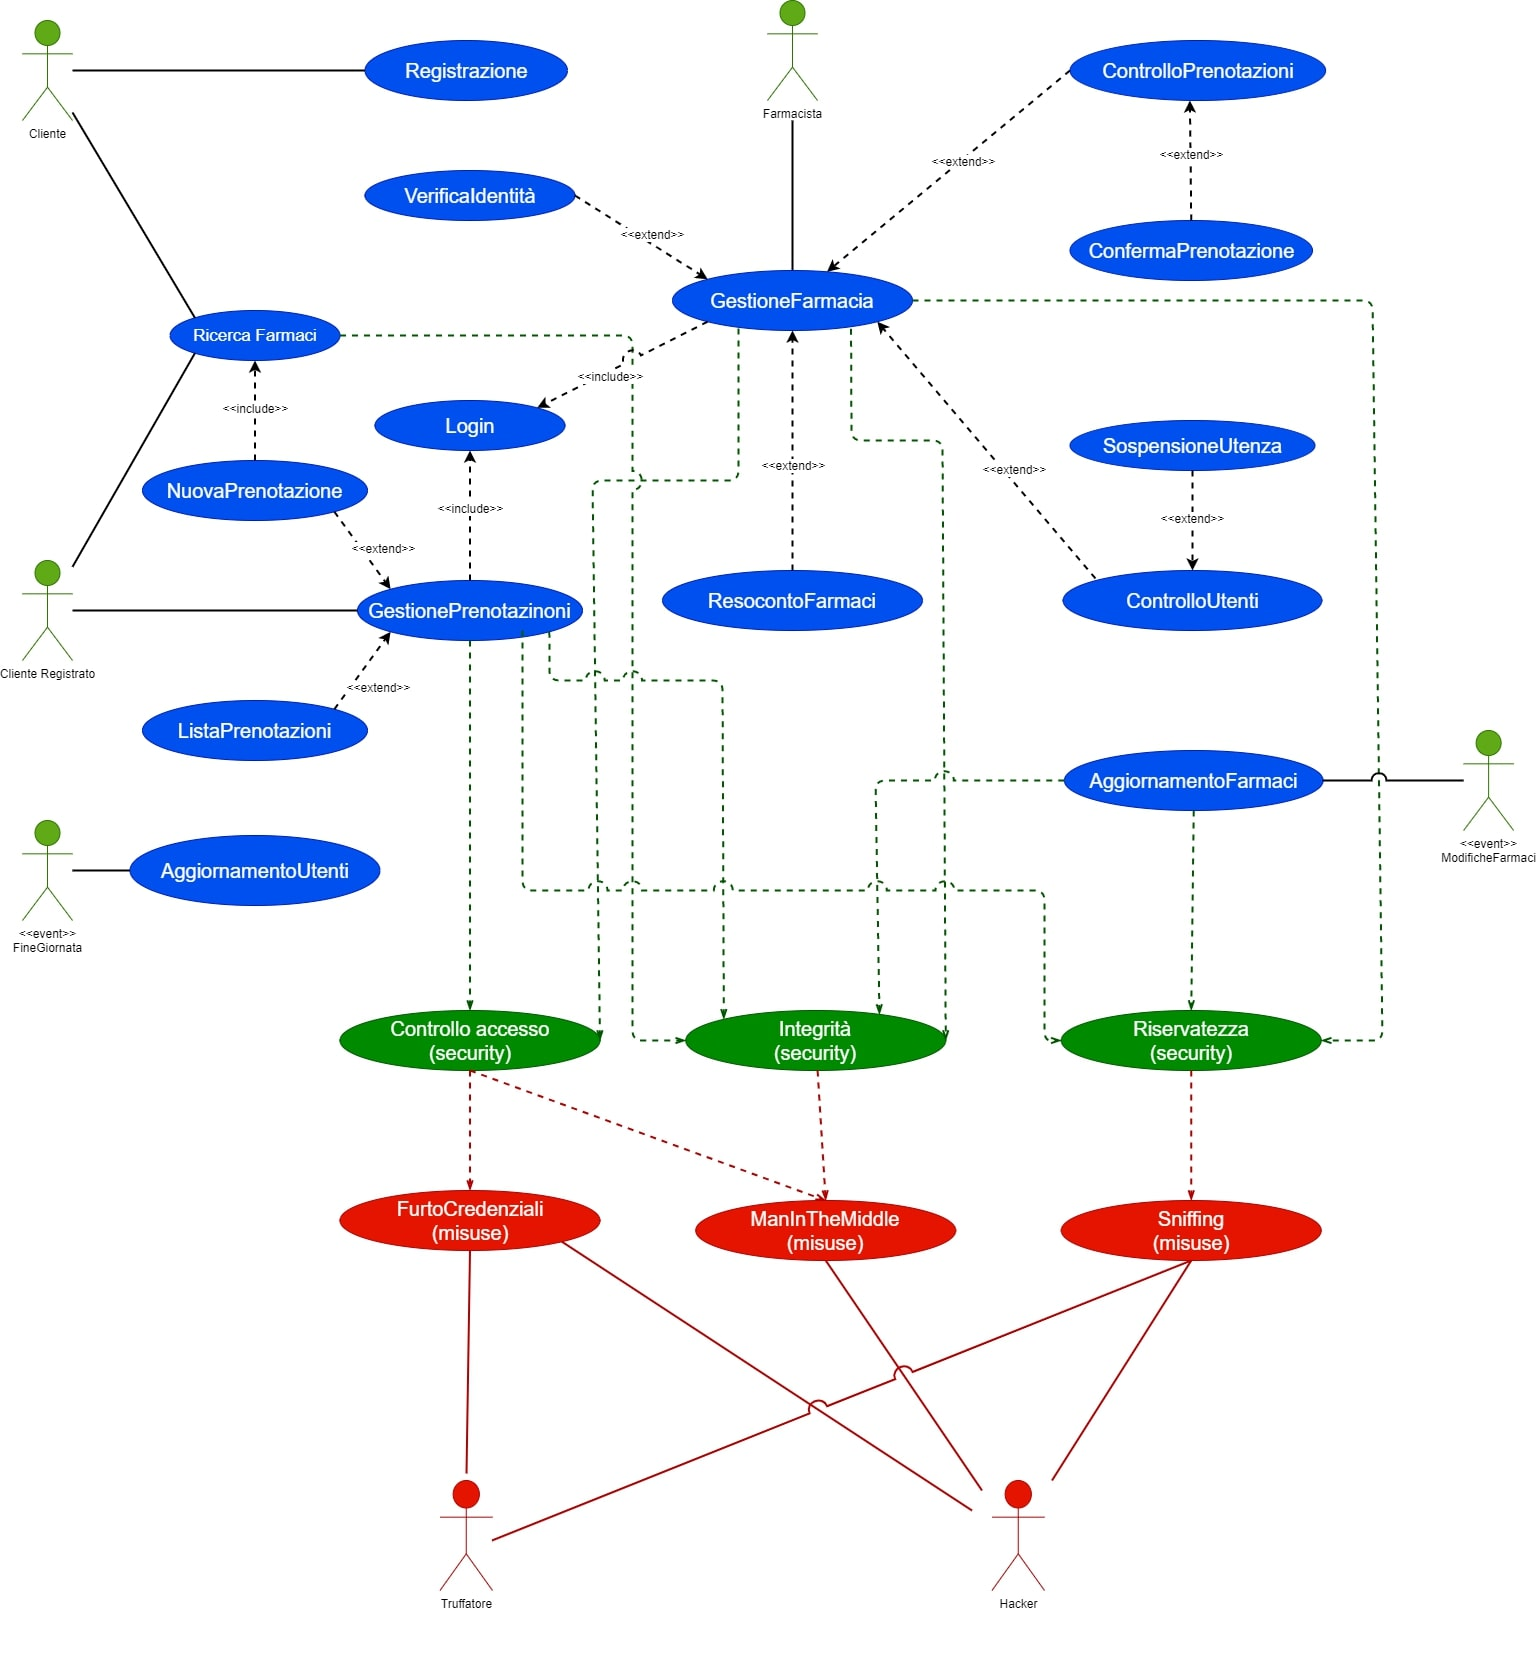
\includegraphics[width=\textwidth]{SecurityCase.jpg}
  \end{center}
\end{figure}
\newpage


\subsubsection{Security Use Case \& Misuse Case Scenari}
\hfill

\begin{tabular} {|P{4cm}|P{13cm}|}
\hline
  \textbf{Titolo} & Riservatezza\\
\hline
  \textbf{Descrizione} & I dati non sono accessibili da chi non ne ha i permessi\\
\hline
  \textbf{Misuse case} & Sniffing\\
\hline
  \textbf{Relazioni} &\\
\hline
  \textbf{Precondizioni} & L'attaccante ha i mezzi per intercettare i messaggi del sistema\\
\hline
  \textbf{Postcondizioni} & Il sistema impedisce all'attaccante di decifrare (in tempi utili) i messaggi intercettati\\
\hline
  \textbf{Scenario principale} & 1. Il Sistema protegge i messaggi \\ 2. L'attaccante riesce ad intercettare un messaggio \\ 3. L'attaccante prova a decifrare i messaggi, ma non riesce a trovare un modo per farlo abbastanza velocemente\\
\hline
  \textbf{Scenari di un attacco avvenuto con successo} & 1. Il Sistema protegge i messaggi \\ 2. L'attaccante riesce ad intercettare un messaggio \\ 3. L'attaccante riesce a decifrare i messaggi e a leggerne il contenuto, ma solamente per una sessione di un utente\\
\hline
\end{tabular}

\hfill
\break

\begin{tabular} {|P{4cm}|P{13cm}|}
\hline
\textbf{Titolo} & Integrità\\
\hline
  \textbf{Descrizione} & Integrità dei dati del sistema\\
\hline
  \textbf{Misuse case} & ManInTheMiddle\\
\hline
  \textbf{Relazioni} &\\
\hline
  \textbf{Precondizioni} & 1. L'attaccante ha i mezzi per intercettare i messaggi del sistema \\ 2. L'attaccante ha i mezzi per modificare i messaggi \\ 3. L'attaccante ha i mezzi per spedire il messaggio modificato al destinatario\\
\hline
  \textbf{Postcondizioni} & Il sistema rileva il messaggio contraffatto\\
\hline
  \textbf{Scenario principale} & 1. Il Sistema protegge i messaggi \\ 2. L'attaccante riesce ad intercettare un messaggio e lo modifica \\ 3. Il sistema si accorge del messaggio contraffatto e lo segna nei log\\
\hline
  \textbf{Scenari di un attacco avvenuto con successo} & 1. Il Sistema protegge i messaggi \\ 2. L'attaccante riesce ad intercettare un messaggio e lo modifica \\ 3. Il sistema accetta il messaggio e agisce di conseguenza, segnando il messaggio nei log\\
\hline
\end{tabular}
\\

\begin{tabular} {|P{4cm}|P{13cm}|}
\hline
  \textbf{Titolo} & ControlloAccessi\\
\hline
  \textbf{Descrizione} & L'accesso alle funzionalità del sistema deve essere controllato\\
\hline
  \textbf{Misuse case} & FurtoCredenziali, ManInTheMiddle\\
\hline
  \textbf{Relazioni} &\\
\hline
  \textbf{Precondizioni} & L'attaccante ha i mezzi per carpire in tutto o in parte le credenziali di accesso di un cliente o di un farmacista\\
\hline
  \textbf{Postcondizioni} & Il sistema blocca l'accesso non autorizzato e notifica il tentativo di accesso\\
\hline
  \textbf{Scenario principale} & 1. L'attaccante tenta di accedere al servizio spacciandosi per un utente legittimo, di cui conosce le credenziali solo in parte (ad esempio mediante attacco con dizionario) \\ 2. Il sistema non riconosce le credenziali, restituendo un errore \\ 3. In seguito ad un numero fissato di tentativi falliti, il sistema blocca temporaneamente l'accesso a quell'utente e notifica l'anomalia a chi di dovere\\
\hline
  \textbf{Scenari di un attacco avvenuto con successo} & 1. L'attaccante riesce a carpire le credenziali di accesso complete di un utente in un qualsiasi modo \\ 2. Il sistema riconosce la correttezza delle credenziali, e fornisce l'accesso al soggetto malevolo 3. L'attaccante ha libero accesso al sistema, con privilegi diversi in base al tipo di utente\\
\hline
\end{tabular}
\\

\subsubsection{Requisiti di Protezione dei Dati}

Sussistono inoltre i seguenti requisiti inerenti alla protezione dei dati: 
\begin{enumerate}
 \item I dati salvati devono essere protetti da un attaccante che abbia accesso al sistema, prendendo misure
di sicurezza fisica, eventualmente cifrando i dati. 
 \item I dati inviati tra le parti remote devono essere protetti, utilizzando la cifratura dei
dati. 
 \item Tutte le azioni avvenute sul sistema devono essere tracciate
tramite un sistema di log. 
\end{enumerate}

\raggedright{La visione e l'analisi dei log verrà gestita
con un editor di testo esterno, accessibile solo al personale
autorizzato.}
\hfill \break

\begin{tabular} {|P{3cm}|P{10cm}|P{3cm}|}
\hline
  \textbf{ID} & \textbf{Requisiti} & \textbf{Tipo}\\
\hline
  R16F & Implementazione di un sistema di log per tracciare tutti i messaggi tra i client e i server, inclusi gli accessi, le richieste di prenotazione, di conferma, di sospensione e di invio e ricezione di dati & Funzionale\\
\hline
  R9NF & I dati salvati devono essere protetti da un attaccante che abbia accesso al sistema, prendendo misure di sicurezza fisica, eventualmente cifrando i dati & Non Funzionale\\
\hline
  R10NF & I dati inviati tra le parti remote devono essere protetti, utilizzando la cifratura dei dati & Non Funzionale\\
\hline
\end{tabular}

\newpage
\section{Analisi del Problema}
\subsection{Analisi Documento dei Requisiti: Analisi delle Funzionalità}
\hfill \break

\textbf{Tabella delle Funzionalità}
\\

\begin{tabular} {|P{4cm}|P{4cm}|P{3.5cm}|P{4cm}|} % Qua cambiate a piacimento la larghezza
    \hline
    \textbf{Funzionalità} & \textbf{Tipo} & \textbf{Grado di complessità} & \textbf{Requisiti Collegati} \\
    \hline
    Gestione Farmacia & Memorizzazione dati e gestione dati & complessa & R5F, R9F, R10F, R11F, R12F, R13F, R14F, R15F \\
    \hline
    Registrazione & Interazione esterno e memorizzazione dati & semplice & R4F \\
    \hline
    RicercaFarmaci  &  Interazione esterno e lettura dati  &  semplice  &   R1F, R2F, R3F \\
    \hline
    Login  &  Interazione esterno e lettura dati  &  semplice  &   R7F \\
    \hline
    GestionePrenotazioni  &  Interazione esterno e memorizzazione dati  &  comp  &   R2F, R6F, R8F \\
    \hline
    ScritturaLog  &  Memorizzazione dati  &  semplice  &   R16F \\
    \hline
\end{tabular}
\\
\hfill \break

\textbf{GestioneFarmacia: Tabella Informazioni/Flusso}
\\

\begin{tabular} {|P{3cm}|P{3cm}|P{3cm}|P{3cm}|P{3cm}|}
    \hline
    \textbf{Informazione} & \textbf{Tipo} & \textbf{Livello protezione/privacy} & \textbf{Input / Output} & \textbf{Vincoli}\\
    \hline
    Nome Cliente & semplice & Protezione alta & Output & Non più di 40 caratteri \\
    \hline
    Cognome Cliente & semplice & Protezione alta & Output & Non più di 40 caratteri \\
    \hline
    Codice Fiscale Cliente & semplice & Protezione media & Output & Deve essere di 16 caratteri \\
    \hline
    Stato Cliente & semplice & Protezione media & Output & \\
    \hline
    Lista Farmaci & composto & Protezione alta & Output & \\
    \hline
    Lista Prenotazioni & composto & Protezione molto alta & Output & \\
    \hline
\end{tabular}
\hfill \break

\newpage
\textbf{Registrazione: Tabella Informazioni/Flusso}
\hfill \break

\begin{tabular} {|P{3cm}|P{3cm}|P{3cm}|P{3cm}|P{3cm}|}
    \hline
    \textbf{Informazione} & \textbf{Tipo} & \textbf{Livello protezione/privacy} & \textbf{Input/Output} & \textbf{Vincoli} \\
    \hline
    Nome Cliente & Semplice & Protezione media & Input & Non più di 40 caratteri \\
    \hline
    Cognome Cliente & semplice & Protezione media & Input & Non più di 40 caratteri \\
    \hline
    Data di Nascita & semplice & Protezione media & Input & Deve avere più di 16 anni e data di nascita successiva al 1900 \\
    \hline
    Codice Fiscale & semplice & Protezione media & Input & Deve essere di 16 caratteri \\
    \hline
    Email &  semplice & Protezione alta & Input & Deve essere di 256 caratteri e del formato giusto \\
    \hline
    Password & semplice & Protezione molto alta & Input & Deve essere almeno di 8 caratteri, di cui uno alfabetico e uno numerico \\
    \hline
\end{tabular}
\hfill \break
\hfill \break

\textbf{ScritturaLog: Tabella Informazioni/Flusso}
\hfill \break

\begin{tabular} {|P{3cm}|P{3cm}|P{3cm}|P{3cm}|P{3cm}|}
    \hline
    \textbf{Informazione} & \textbf{Tipo} & \textbf{Livello protezione/privacy} &  \textbf{Input/Output} & \textbf{Vincoli} \\
    \hline
    Data  & semplice & Protezione media & Input & Non più di 40 caratteri \\
    \hline
    Ora & semplice & Protezione media & Input & Non più di 40 caratteri \\
    \hline
    Attore & semplice & Protezione alta & Input & Non più di 20 caratteri \\
    \hline
    Identificativo Farmacia & semplice & Protezione alta & Input & Non più di 20 caratteri \\
    \hline
    Operazione Eseguita & composto & Protezione alta & Input & \\
    \hline
    Evento & composto & Protezione molto alta & Input &  \\
    \hline
\end{tabular}
\hfill \break
\hfill \break

\textbf{AnalisiLog: Tabella Informazioni/Flusso}
\hfill \break

\begin{tabular} {|P{3cm}|P{3cm}|P{3cm}|P{3cm}|P{3cm}|}
    \hline
    \textbf{Informazione} & \textbf{Tipo} & \textbf{Livello protezione/privacy} & \textbf{Input/Output} & \textbf{Vincoli} \\
    \hline
    Notifica & composto & Protezione bassa & Output &  \\
    \hline
\end{tabular}

\textbf{Login: Tabella Informazioni/Flusso}
\hfill \break

\begin{tabular} {|P{3cm}|P{3cm}|P{3cm}|P{3cm}|P{3cm}|}
    \hline
    \textbf{Informazione} & \textbf{Tipo} & \textbf{Livello protezione/privacy} & \textbf{Input/Output} & \textbf{Vincoli} \\
    \hline
    Email & semplice & Protezione molto alta & Input & Non più di 256 caratteri \\
    \hline
    Password & semplice & Protezione molto alta & Input & Non più di 50 caratteri \\
    \hline
\end{tabular}
\hfill \break
\hfill \break

\textbf{GestionePrenotazione: Tabella Informazioni/Flusso}
\hfill \break

\begin{tabular} {|P{3cm}|P{3cm}|P{3cm}|P{3cm}|P{3cm}|}
    \hline
    \textbf{Informazione} & \textbf{Tipo} & \textbf{Livello protezione/privacy} & \textbf{Input/Output} & \textbf{Vincoli} \\
    \hline
    Data invio & semplice & Protezione media & Input & Non più di 40 caratteri \\
    \hline
    Ora invio & semplice & Protezione media & Input & Non più di 40 caratteri \\
    \hline
    Data prenotazione & semplice & Protezione media & Input & Solo una data compresa tra il giorno successivo e 14 giorni dopo \\
    \hline
    Elenco farmaci & composto & Protezione alta & Input & 1. Non più di 5 elementi per ogni farmaco <br> 2. Non più di 20 elementi in totale \\
    \hline
    Identificativo farmacia & semplice & Protezione alta & Input & Non più di 20 caratteri \\
    \hline
    Identificativo cliente & semplice & Protezione molto alta & Input & Non più di 20 caratteri \\
    \hline
    Lista prenotazioni  &  composto  &  Protezione alta  &  Output  &  \\
    \hline
\end{tabular}

\newpage
\subsubsection{Analisi Documento dei Requisiti: Analisi dei Vincoli}
\hfill \break

\textbf{Tabella Vincoli}
\hfill \break

\begin{tabular} {|P{3cm}|P{2.5cm}|P{3.5cm}|P{6cm}|}
    \hline
    \textbf{Requisito} & \textbf{Categorie} & \textbf{Impatto} & \textbf{Funzionalità} \\
    \hline
    Semplicità dell'interfaccia & Usabilità & Intuitività di utilizzo &  GestioneFarmacia, Registrazione, RicercaFarmaci, Login, NuovaPrenotazione  \\
    \hline
    Velocità della ricerca dei dati & Tempo di Risposta & Maggiore reattività & GestioneFarmacia, Registrazione, RicercaFarmaci, Login, NuovaPrenotazione \\
    \hline
    Velocità di memorizzazione dei dati & Tempo di Risposta & Maggiore reattività & GestioneFarmacia, Registrazione, Login, NuovaPrenotazione \\
    \hline
    Controllo Accessi &  Sicurezza  &  Peggiorano tempo di risposta e usabilità, migliorano la privacy dei dati  &  GestioneFarmacia, NuovaPrenotazione  \\
    \hline
    Protezione dei Dati &  Sicurezza  &  Peggiorano tempo di risposta, migliorano la privacy dei dati  &  GestioneFarmacia, Registrazione, RicercaFarmaci, Login, NuovaPrenotazione  \\
    \hline
\end{tabular}

\newpage

\subsubsection{Analisi Documento dei Requisiti: Analisi delle Interazioni}
\hfill \break

\textbf{Tabella Maschere}
\hfill \break

\begin{tabular} {|P{3.5cm}|P{7cm}|P{5cm}|}
    \hline
    \textbf{Maschera} & \textbf{Informazioni} & \textbf{Funzionalità} \\
    \hline
    Home Gestione & messaggio di benvenuto e scelta della funzionalità & GestioneFarmacia \\
    \hline
    View Login & email, password & Login \\
    \hline
    View Prenotazioni & lista prenotazioni & GestioneFarmacia \\
    \hline
    View ResocontoUtenti & nome cliente, cognome cliente, codice fiscale cliente, stato cliente & GestioneFarmacia \\
    \hline
    View VerificaIdentità & nome cliente, cognome cliente, codice fiscale cliente  & VeriticaIdentità \\
    \hline
    View Farmaci & lista farmaci & gestioneFarmacia \\
    \hline
    Home Servizio & messaggio di benvenuto, nome farmaco, località utente, lista farmacie pertinenti & RicercaFarmaci \\
    \hline
    View Registrazione &  nome cliente, cognome cliente, data di nascita, codice fiscale, email, password  & Registrazione \\
    \hline
    View NuovaPrenotazione & data invio, ora invio, data prenotazione, elenco farmaci, identificativo farmacia, identificativo cliente & NuovaPrenotazione \\
    \hline
    View PrenotazioniPersonali & lista prenotazioni & ListaPrenotazioni \\
    \hline
\end{tabular}
\hfill \break
\hfill \break

\textbf{Tabella Sistemi Esterni}
\hfill \break

\begin{tabular} {|P{3cm}|P{4cm}|P{4cm}|P{4cm}|}
    \hline
    \textbf{Sistema} & \textbf{Descrizione} & \textbf{Protocollo di Interazione} & \textbf{Livello di Sicurezza} \\
    \hline
    Gestione Magazzino  &  Sistema che si occupa della gestione dei farmaci in magazzino  &  GestioneMagazzino mette a disposizione delle funzionalità di elencazione dei farmaci  & Medio livello di sicurezza perchè protegge i dati della farmacia  \\
    \hline
\end{tabular}
\hfill \break

\newpage
\subsubsection{Analisi Ruoli e Responsabilità}
\hfill \break

\textbf{Tabella Ruoli}
\hfill \break

\begin{tabular} {|P{2.5cm}|P{3cm}|P{3.5cm}|P{3cm}|P{3cm}|}
    \hline
    \textbf{Ruolo} & \textbf{Responsabilità} & \textbf{Maschere} & \textbf{Riservatezza} & \textbf{Numerosità} \\
    \hline
    Farmacista & Gestione di tutte le informazioni relative agli utenti e alle prenotazioni di una farmacia & Home Gestione, View Login, View Prenotazioni, View ResocontoUtenti, View VerificaIdentità, View Farmaci,  & È richiesto un alto grado di riservatezza  & Massimo 10 farmacisti per ogni farmacia \\
    \hline
    Cliente & Ricerca di un farmaco senza necessità di login & Home Servizio, View Login, View Registrazione  & È richiesto un medio grado di riservatezza & Illimitati \\
    \hline
    % roba molto brutta ma non so perchè non va a capo automaticamente questo
    ClienteRegi- strato & Ricerca e prenotazione di farmaci presso una farmacia & Home Servizio, View NuovaPrenotazione, View PrenotazioniPersonali &  È richiesto un alto grado di riservatezza  & Illimitati \\
    \hline
\end{tabular}
\hfill \break
\hfill \break

\textbf{Farmacista: Tabella Ruolo-Informazioni}
\hfill \break

\begin{tabular} {|P{7cm}|P{7cm}|}
    \hline
    \textbf{Informazione} & \textbf{Tipo di Accesso} \\
    \hline
    Nome Cliente & Lettura \\
    \hline
    Cognome Cliente & Lettura \\
    \hline
    Codice Fiscale & Lettura \\
    \hline
    Stato Cliente & Lettura/Scrittura \\
    \hline
    Lista Farmaci & Lettura/Scrittura \\
    \hline
    Lista Prenotazioni & Lettura/Scrittura \\
    \hline
\end{tabular}
\hfill \break
\hfill \break

\textbf{ClienteRegistrato: Tabella Ruolo-Informazioni}
\hfill \break

\begin{tabular} {|P{7cm}|P{7cm}|}
    \hline
    \textbf{Informazione} & \textbf{Tipo di Accesso} \\
    \hline
    Nome Cliente & Lettura/Scrittura \\ 
    \hline
    Cognome Cliente & Lettura/Scrittura \\
    \hline
    Data di Nascita & Lettura \\
    \hline
    Codice Fiscale & Lettura \\
    \hline
    Email & Lettura/Scrittura \\
    \hline
    Password & Lettura/Scrittura \\
    \hline
    Nome Farmaco & Scrittura \\
    \hline
    Località Utente & Lettura \\
    \hline
    Lista Farmacie Pertinenti  & Lettura \\
    \hline
    Data prenotazione & Scrittura \\
    \hline
    Elenco farmaci & Scrittura \\
    \hline
\end{tabular}

\textbf{Cliente: Tabella Ruolo-Informazioni}
\hfill \break

\begin{tabular} {|P{7cm}|P{7cm}|}
    \hline
    \textbf{Informazione} & \textbf{Tipo di Accesso} \\
    \hline
    Nome Farmaco & Scrittura \\
    \hline
    Località Utente & Scrittura \\
    \hline
    Lista Farmacie Pertinenti  & Lettura \\
    \hline
\end{tabular}
\hfill \break
\hfill \break

\subsubsection{Scomposizione del Problema}
\hfill \break

\textbf{Tabella Scomposizione Funzionalità}
\hfill \break

\begin{tabular} {|P{7cm}|P{7cm}|}
    \hline
    \textbf{Funzionalità} & \textbf{Scomposizione} \\
    \hline
    GestioneFarmacia &  ResocontoFarmaci, ResocontoUtenti, ControlloPrenotazioni, VerificaIdentità  \\
    \hline
    GestionePrenotazioni  &  NuovaPrenotazione, ListaPrenotazioni  \\
    \hline
    ControlloPrenotazioni  &  ConfermaPrenotazione  \\
    \hline
    ResocontoUtenti &  SospensioneUtenza  \\
    \hline
\end{tabular}
\\

Non sono presenti legami di esclusione o di necessità tra le sotto-funzionalità del sistema. 
\hfill \break

\newpage
\subsubsection{Creazione Modello del Dominio}

Il seguente diagramma delle classi rappresenta la parte di modello del dominio relativa al sistema. \\

\begin{figure}[h!]
    \begin{center}
        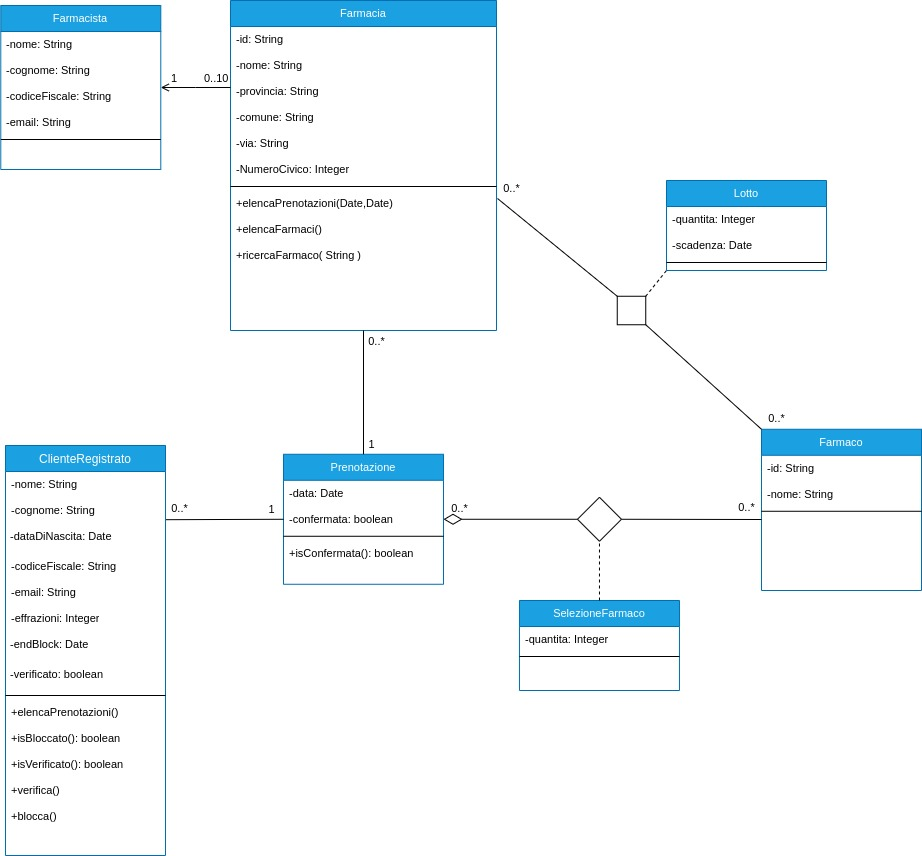
\includegraphics[width=\textwidth]{immagini/ModelloDominio.jpg}
    \end{center}
\end{figure}
\hfill \break

\newpage
\subsubsection{Architettura Logica: Struttura}
\hfill \break

\textbf{Diagramma dei package}
\hfill \break

\begin{figure}[h!]
    \begin{center}
        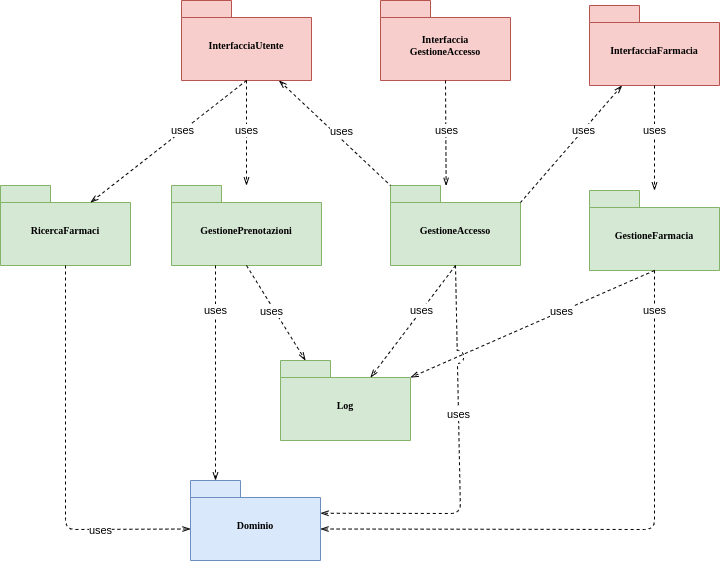
\includegraphics[scale=0.6]{immagini/Diagrammi-Package.png}
    \end{center}
\end{figure}
\hfill \break

\textbf{Diagramma delle classi: GestioneAccesso}
\hfill \break

\begin{figure}[h!]
    \begin{center}
        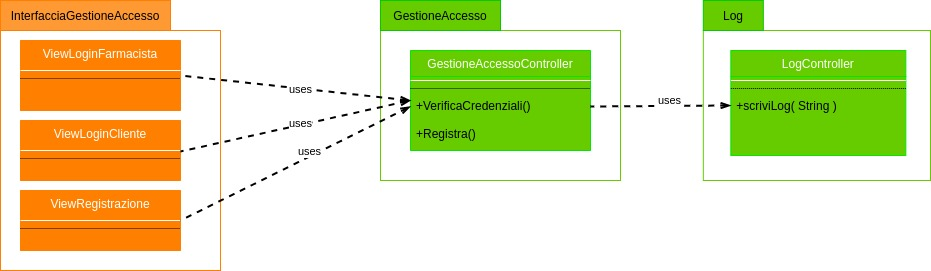
\includegraphics[width=\textwidth]{immagini/Diagrammi-Gestione Accesso.jpg}
    \end{center}
\end{figure}
\hfill \break

\textbf{Diagramma delle classi: Gestione Farmacia \& Interfaccia Farmacia}
\hfill \break

\begin{figure}[h!]
    \begin{center}
        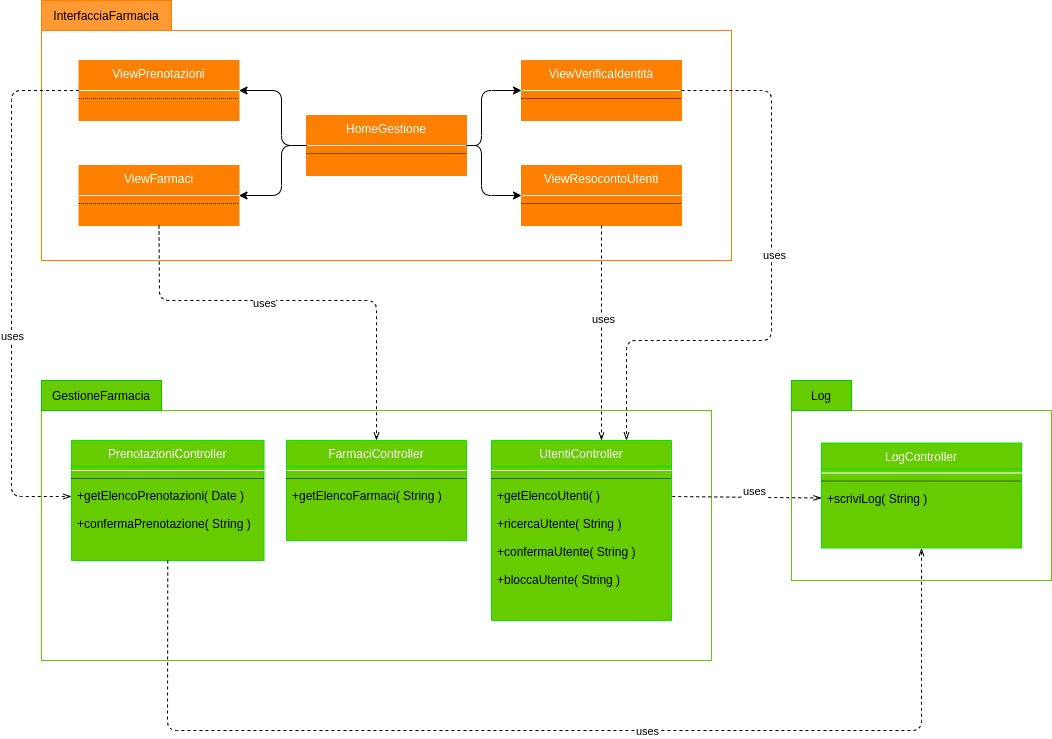
\includegraphics[width=\textwidth]{immagini/Diagrammi-Farmacia.jpg}
    \end{center}
\end{figure}
\hfill \break

\newpage
\textbf{Diagramma delle classi: Interfaccia Utente}

\begin{figure}[h!]
    \begin{center}
        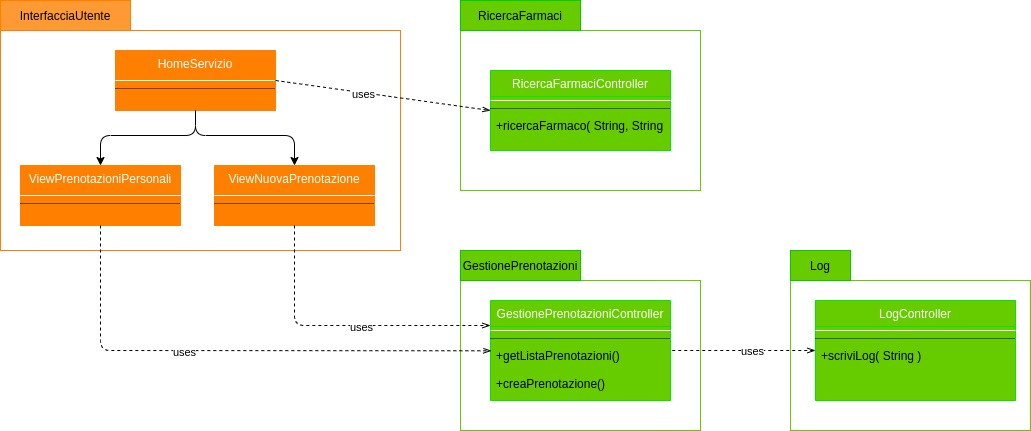
\includegraphics[width=\textwidth]{immagini/Diagrammi-Utente.jpg}
    \end{center}
\end{figure}
\hfill \break

\newpage
\subsubsection{Architettura Logica: Interazione}
\hfill \break

\textbf{Diagramma di Sequenza: Login Utente}

\begin{figure}[h!]
    \begin{center}
        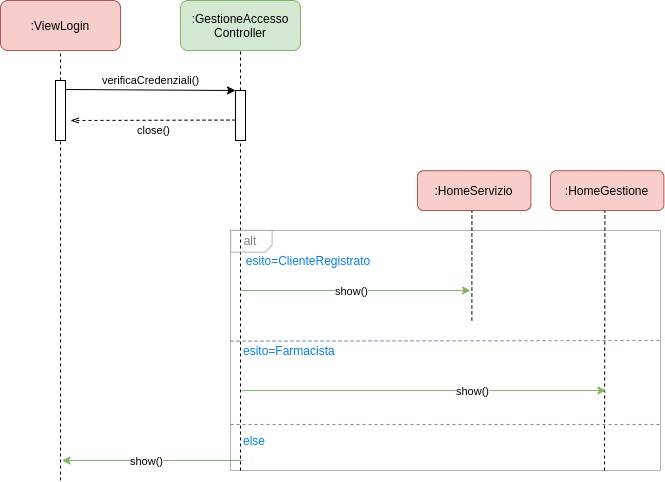
\includegraphics[scale=0.5]{immagini/Interazione-LoginUtente.jpg}
    \end{center}
\end{figure}
\hfill \break

\textbf{Diagramma di Sequenza: Registrazione Utente}

\begin{figure}[h!]
    \begin{center}
        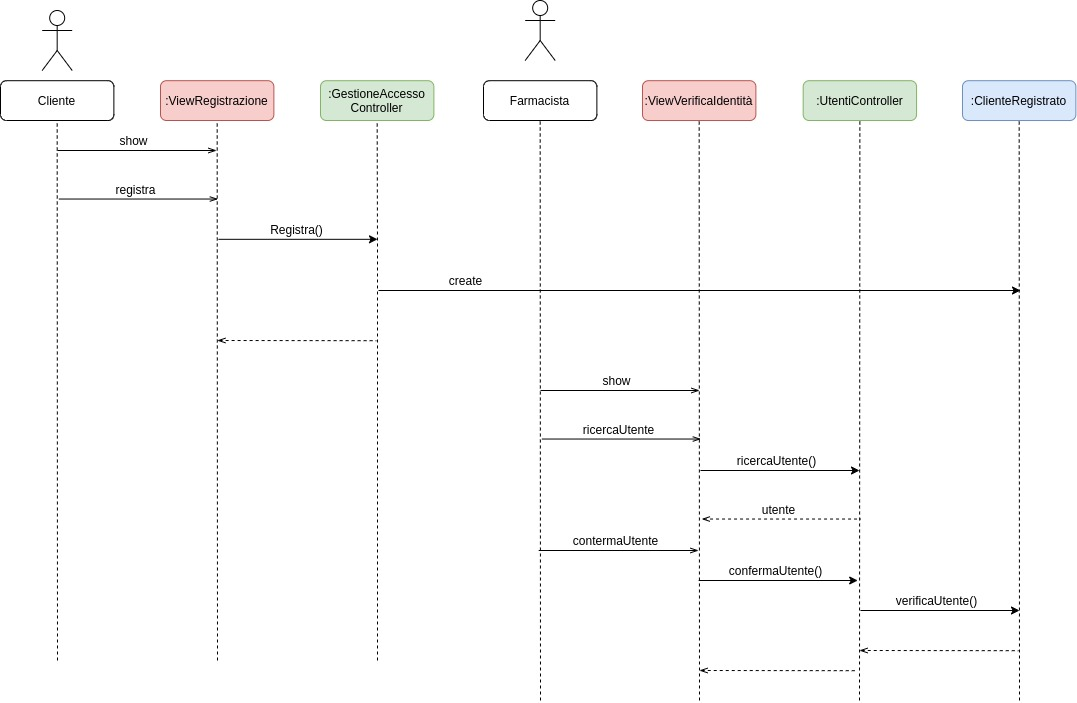
\includegraphics[scale=0.4]{immagini/Interazione-RegistrazioneUtente.jpg}
    \end{center}
\end{figure}
\hfill \break

\textbf{Diagramma di Sequenza: Nuova Prenotazione}

\begin{figure}[h!]
    \begin{center}
        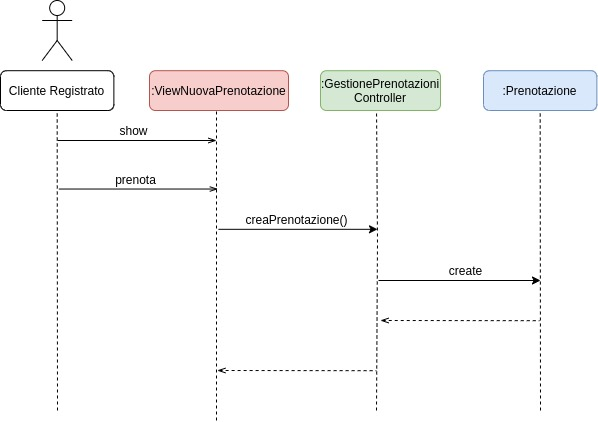
\includegraphics[scale=0.5]{immagini/Interazione-NuovaPrenotazione.jpg}
    \end{center}
\end{figure}
\hfill \break

\textbf{Diagramma di Sequenza: Conferma Prenotazione}

\begin{figure}[h!]
    \begin{center}
        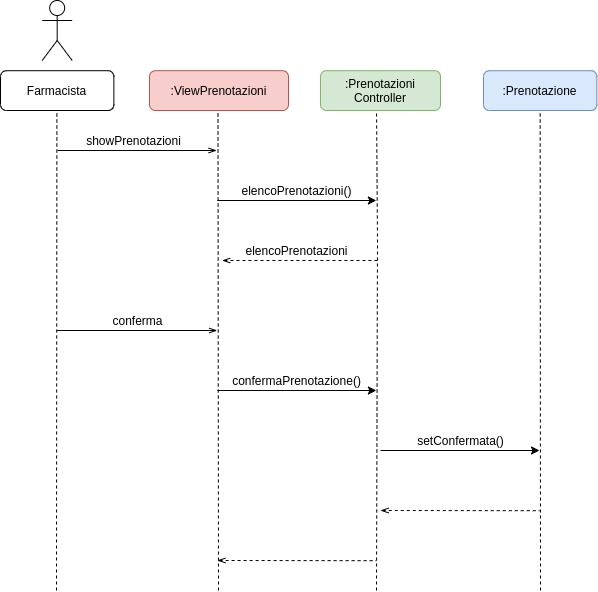
\includegraphics[scale=0.5]{immagini/Interazione-ConfermaPrenotazione.jpg}
    \end{center}
\end{figure}
\hfill \break

\textbf{Diagramma di Sequenza: Ricerca Farmaco}

\begin{figure}[h!]
    \begin{center}
        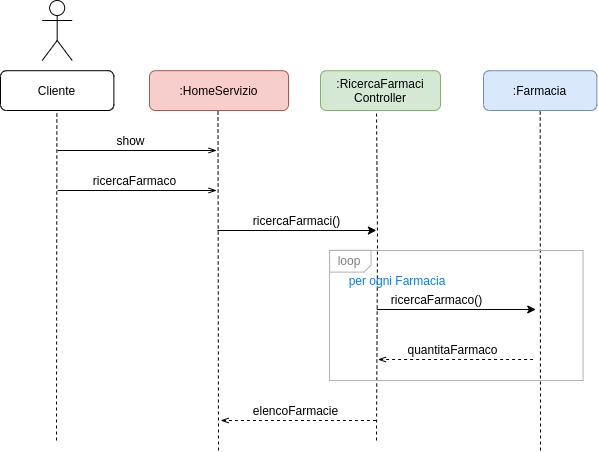
\includegraphics[scale=0.5]{immagini/Interazione-RicercaFarmaco.jpg}
    \end{center}
\end{figure}
\hfill \break

\textbf{Diagramma di Sequenza: Sospensione Utenza}

\begin{figure}[h!]
    \begin{center}
        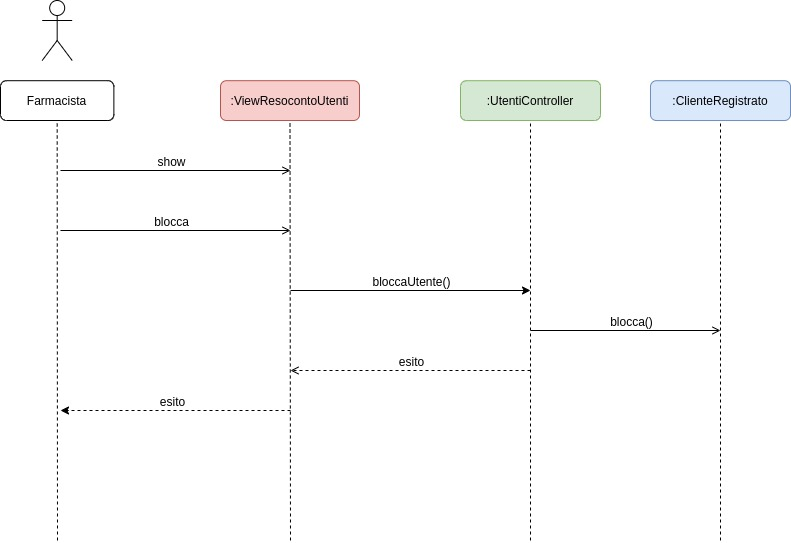
\includegraphics[scale=0.5]{immagini/Interazione-SospensioneUtenza.jpg}
    \end{center}
\end{figure}
\hfill \break

\newpage
\subsubsection{Architettura Logica: Comportamento}
\hfill \break

\textbf{Diagramma di Stato: Analizza Utente}

\begin{figure}[h!]
    \begin{center}
        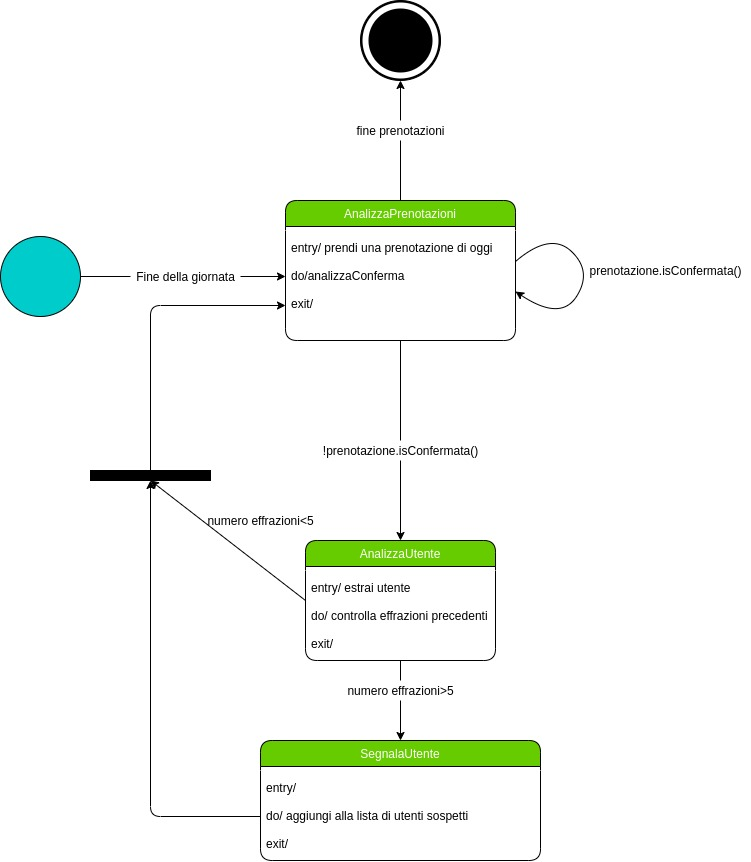
\includegraphics[scale=0.5]{immagini/Comportamento.jpg}
    \end{center}
\end{figure}
\hfill \break

\newpage
\subsubsection{Piano di Lavoro}

I compiti sono stati divisi in base alle competenze di 
ogni membro del gruppo come indicato nella tabella sottostante:\\

\begin{tabular} {|P{5cm}|P{5cm}|P{5cm}|} % Qua cambiate a piacimento la larghezza
    \hline
    \textbf{Package} & \textbf{Progetto} & \textbf{Sviluppo} \\
    \hline
    Dominio  &  Guerra,Palaferri,Romanini  &  Guerra\\
    \hline
    Log  &  Guerra,Palaferri,Romanini & Guerra\\
    \hline
    RicercaFarmaci  &  Guerra,Palaferri,Romanini &  Palaferri \\
    \hline
    GestionePrenotazioni  & Guerra,Palaferri,Romanini & Palaferri,Romanini \\
    \hline
    GestioneAccesso  & Guerra,Palaferri,Romanini & Guerra,Romanini \\
    \hline
    GestioneFarmacia  & Guerra,Palaferri,Romanini & Palaferri,Romanini \\
    \hline
    InterfacciaUtente  & Guerra,Palaferri,Romanini & Romanini \\
    \hline
    InterfacciaGestioneAccsso  & Guerra,Palaferri,Romanini & Guerra\\
    \hline
    InterfacciaFarmacia  & Guerra,Palaferri,Romanini & Palaferri,Romanini \\
    \hline
\end{tabular}
\hfill \break

I tempi di rilascio sono i seguenti:
\begin{itemize}
    \item Progettazione entro due settimane dalla data di odierna
    \item Sviluppo dei vai moduli con annessi test unitari entro una settimana dalla fine della fase di progettazione
    \item Integrazione e testing del sistema entro una settimane dalla fine dello sviluppo
\end{itemize}
\hfill \break

\textbf{Sviluppi Futuri}
\\

Il cliente ha richiesto la creazione di un applicativo mobile per sistemi
android e iOS, con l'obbiettivo di rendere il più pratico possibile l'utilizzo
del programma.

\newpage
\subsubsection{Piano del Collaudo}

\usemintedstyle{manni}
\begin{minted}
[
frame=lines,
framesep=2mm,
baselinestretch=1.2,
bgcolor=LightGray,
fontsize=\footnotesize,
linenos
]
{java}
public class testPrenotazione{
    private Prenotazione prenotazione;

    @Before
    public void setUp(){
       prenotazione = new Prenotazione();
    }

    @Test
    public void testCostruttore(){
        prenotazione = new Prenotazione(new SimpleDateFormat("2021-06-01"), true);
        Assert.assertNull(prenotazione.isConfermata());
    }

    @Test
    public void testGetter(){
        prenotazione = new Prenotazione(new SimpleDateFormat("2021-06-01"), true);
        Assert.assertEquals(prenotazione.getData(), new SimpleDateFormat("2021-06-01"));
        Assert.assertEquals(prenotazione.getConfermata(), true);
    }

    @Test
    public void testSetter(){
        prenotazione.setData(new SimpleDateFormat("2021-07-02"));
        Assert.assertEquals(prenotazione.getData(), new SimpleDateFormat("2021-07-02"));
        prenotazione.setConfermata(true);
        Assert.assertEquals(prenotazione.getConfermata(), true);
    }
}

public class testFarmacia{
    private Farmacia farmacia;

    @Before 
    public void setUp(){
        farmacia = new Farmacia();
    }

    @Test
    public void testCostruttore(){
        Assert.assertNull(farmacia.getNome());
        Assert.assertNull(farmacia.getId());
    }

    @Test 
    public void testGetter(){
        farmacia = new Farmacia("N23N230SD", "Ubertini", "BO", "Bologna", "via Libia", "10");
        Assert.assertEquals(farmacia.getId(),"N23N230SD");
        Assert.assertEquals(farmacia.getNome(),"Ubertini");
        Assert.assertEquals(farmacia.getProvincia(),"BO");
        Assert.assertEquals(farmacia.getComune(),"Bologna");
        Assert.assertEquals(farmacia.getVia(),"via Libia");
        Assert.assertEquals(farmacia.getNumeroCivico(),"10");
    }

    @Test 
    public void testSetter(){
        farmacia.setId("N23N230SD");
        Assert.assertEquals(farmacia.getId(),"N23N230SD");
        farmacia.setNome("Ubertini");
        Assert.assertEquals(farmacia.getNome(),"Ubertini");
        farmacia.setProvincia("BO");
        Assert.assertEquals(farmacia.getProvincia(),"BO");
        farmacia.setComune("Bologna");
        Assert.assertEquals(farmacia.getComune(),"Bologna");
        farmacia.setVia("via Libia");
        Assert.assertEquals(farmacia.getVia(),"via Libia");
        farmacia.setNumeroCivico("10");
        Assert.assertEquals(farmacia.getNumeroCivico(),"10");
    }
}

public class testCliente{
    private ClienteRegistrato cliente;

    @Before 
    public void setUp(){
        cliente = new ClienteRegistrato();
    }

    @Test 
    public void testGetter(){
        cliente = new ClienteRegistrato("Federico", "Chesani", new
        SimpleDateFormat("1920-07-10"), "CHSFRC20L10A944G",
        "federico.chesani@unibo.it", 0, null, true, false);
        Assert.assertEquals(cliente.getNome(), "Federico");
        Assert.assertEquals(cliente.getCognome(), "Chesani");
        Assert.assertEquals(cliente.getNascita(), new SimpleDateFormat("1920-07-10"));
        Assert.assertEquals(cliente.getCodiceFiscale(), "CHSFRC20L10A944G");
        Assert.assertEquals(cliente.getEmail(), "federico.chesani@unibo.it");
        Assert.assertEquals(cliente.getEffrazioni(), 0);
        Assert.assertEquals(cliente.getVerificato(), true);
        Assert.assertEquals(cliente.getBloccato(), false);
    }

    @Test 
    public void testSetter(){
        cliente.setNome("Federico");
        Assert.assertEquals(cliente.getNome(), "Federico");
        cliente.setCognome("Chesani");
        Assert.assertEquals(cliente.getCognome(), "Chesani");
        cliente.setNascita(new SimpleDateFormat("1920-07-10"));
        Assert.assertEquals(cliente.getNascita(), new SimpleDateFormat("1920-07-10"));
        cliente.setCodiceFiscale("CHSFRC20L10A944G");
        Assert.assertEquals(cliente.getCodiceFiscale(), "CHSFRC20L10A944G");
        cliente.setEmail("federico.chesani@unibo.it");
        Assert.assertEquals(cliente.getEmail(), "federico.chesani@unibo.it");
        cliente.setEffrazioni(0);
        Assert.assertEquals(cliente.getEffrazioni(), 0);
        cliente.setVerificato(true);
        Assert.assertEquals(cliente.getVerificato(), true);
        cliente.setBloccato(false);
        Assert.assertEquals(cliente.getBloccato(), false);
    }
}
\end{minted}

\newpage
\section{Progettazione}

\subsection{Progettazione Architetturale}

\subsubsection{Requisiti non funzionali}

Dall'analisi dei requisiti sono emersi i seguenti requisiti non funzionali:
\begin{itemize}
\item Tempo di risposta
\item Usabilità
\item Integrità dei dati
\item Protezione dei dati 
\item Sicurezza delle comunicazioni
\end{itemize}
La protezione dei dati e delle comunicazioni assume fondamentale importanza vista la natura del software, 
che deve trattare dati personali e sanitari dei clienti. 
La compromissione di questi risulterebbe in una grave perdita finanziaria e di immagine, senza considerare i danni apportati alla privacy degli utenti. 
Inoltre, sarà necessario assicurare la sicurezza fisica dei dati immagazzinati nel sistema.
L'introduzione di misure di sicurezza delle comunicazioni e protezione dei dati non compromette l'usabilità del sistema, ma potrebbe peggiorarne leggerlmente le prestazioni: 
è possibile comunque bilanciare le due esigenze senza eccessive complicazioni mediante le tecnologie esposte in seguito. 
Va notato inoltre che il sistema non presenta vincoli di tempo particolarmente stringenti (nessun vincolo real-time).


\subsubsection{Scelta dell'architettura}

Dopo una rapida analisi, si è constatato che l'architettura più adeguata per il sistema è l'\textbf{architettura client-server a 3 livelli}.

\paragraph{L1 -- Client}\mbox{}\\ \\
La componente lato Client sarà implementata da due interfacce differenti:

\begin{itemize}
\item[-] Un'interfaccia per le funzionalità relative ai clienti (registrati e non)
\item[-] Un'interfaccia per la gestione della farmacia da parte di un operatore (farmacista)
\end{itemize}

\paragraph{L2 -- Server}\mbox{}\\ \\
Rispettando il principio del "minimo privilegio" per limitare i danni in caso di attacco e per distribuire meglio il carico, si è deciso di scomporre i server in base alle funzionalità offerte. Si hanno quindi tre server:

\begin{itemize}
\item[-] Un server che fornisce i servizi ai clienti registrati e non
\item[-] Un server che funge da pannello di controllo per i farmacisti
\item[-] Un server per le funzionalità di autenticazione
\end{itemize}

\paragraph{L3 -- Persistenza}\mbox{}\\ \\
La gestione della persistenza verrà implementata in un server dedicato sul quale sarà installato un DBMS che gestisca i dati di tutte le farmacie aderenti al servizio.
L'interfacciamento con il DBMS avverrà mediante la metodologia "forza bruta" utilizzando i metodi CRUD.
Per quanto riguarda il log delle operazioni, invece, questo verrà salvato su file system (un semplice file sul server adibito)

\subsubsection{Pattern architetturali e di design}

Infine, dopo un'attenta analisi, si è optato per l'adozione del pattern \textbf{Broker}: 
un componente verrà interposto alla comunicazione Client--Server e avrà il compito di indirizzare le richieste dei client al relativo server, 
effettuando un controllo sulle sessioni attive per determinare lo stato del client. 
La scomposizione in diversi client e server consente di avere una separazione netta tra gli applicativi del cliente e del farmacista, 
in modo da localizzare le operazioni critiche e ottenere maggiore protezione dei dati.
Il pattern Model View Controller (\textbf{MVC}) è stato invece scelto come pattern architetturale.
\\
Chiaramente l'affidabilità del sistema dipende dalla robustezza del broker e soprattutto del sistema di autenticazione.
\\ \\
Si riportano di seguito i diagrammi di package e componenti che descrivono l'architettura del sistema.

\begin{figure}[h]
    \begin{center}
        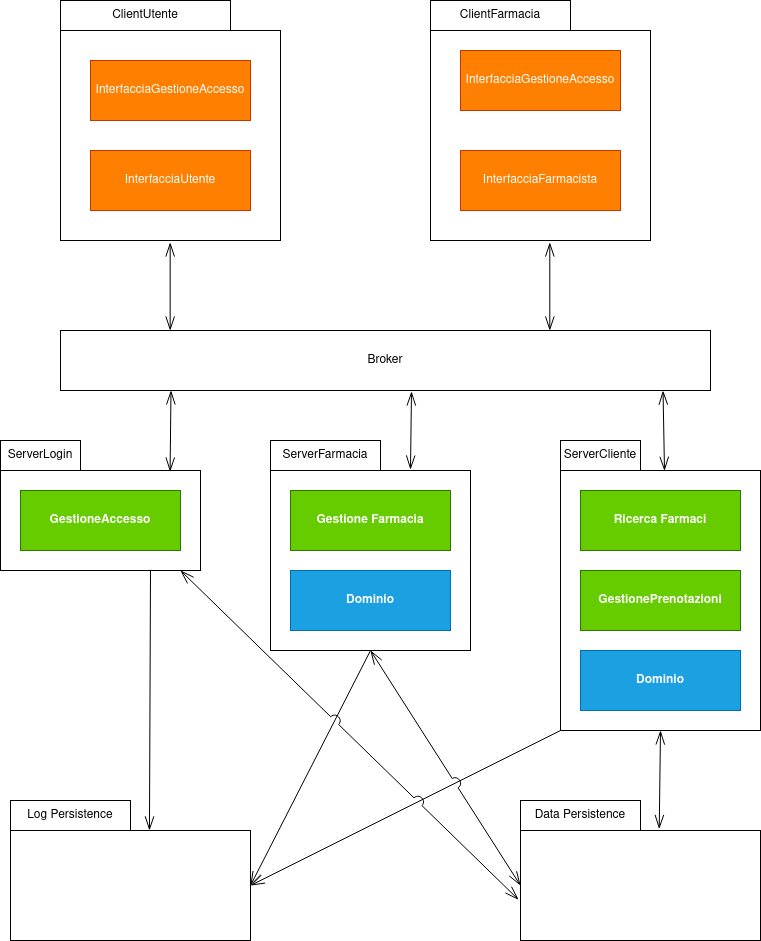
\includegraphics[scale=0.4]{immagini/Package-progettazione.png}
        \caption{Diagramma dei package}
    \end{center}
\end{figure}


\end{document}
